\documentclass[11pt,a4paper]{report}
\usepackage[utf8]{inputenc}
\usepackage[T1]{fontenc}
\usepackage{alltt}
\usepackage{graphicx}
\usepackage{hyperref}
\usepackage{scrextend}
\usepackage{enumitem}

% Changed the section command to say "Task #"
\def\thesection{Task \arabic{section}:}
% Added a familiar HTML command for new paragraph
\newcommand{\p}{\medskip\noindent}

% Meta, should be edited and filled in with relative information
\title{TDT4230 Graphics and Visualisation \\\\ Assignment 1}

\author{Nikola Dordevic}
\date{\today}

\begin{document}
% Use \section for tasks
\section{Let there be light [2.0 points]}
\begin{enumerate}[label=(\alph*)]\setcounter{enumi}{9}
	\item 3 Point Lights: \\ \hspace*{5mm} 2 in the box node \\ \hspace*{5mm} 1 in the ball node
	
	
	\begin{figure}[h]
		\centering
		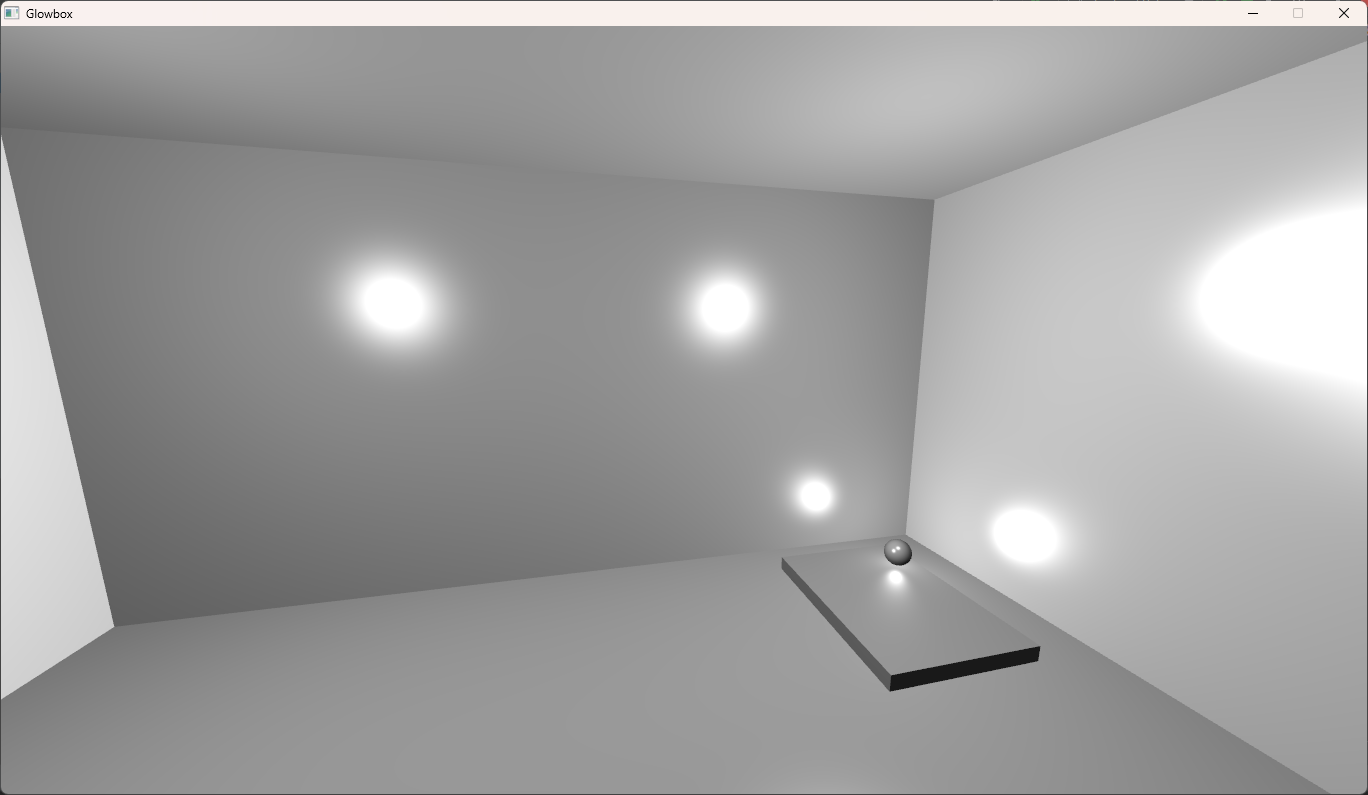
\includegraphics[width=\textwidth]{images/task1j.png}
		\caption{Screenshot of Glowbox with Phong lighting}
	\end{figure}
	
	
	
\end{enumerate}

% Command for next page
\clearpage

\section{}
% This is how to place two screenshots side by side for comparison

\end{document}